% !TeX program = xelatex
% COSTTRACE research manuscript draft
% This manuscript skeleton is evidence-based and uses only metrics/artifacts
% present in the repository as of 2026-06-24.

\documentclass[11pt,a4paper]{article}

\usepackage[a4paper,margin=1in]{geometry}
\usepackage{iftex}
\ifPDFTeX
  \usepackage[T1]{fontenc}
  \usepackage[utf8]{inputenc}
  \usepackage{newtxtext,newtxmath}
\else
  \usepackage{fontspec}
  \setmainfont{Times New Roman}
  \setsansfont{Arial}
  \setmonofont{Consolas}
\fi

\usepackage{setspace}
\doublespacing
\usepackage{microtype}
\usepackage{amsmath,amssymb}
\usepackage{graphicx}
\usepackage{booktabs}
\usepackage{array}
\usepackage{tabularx}
\usepackage{longtable}
\usepackage{caption}
\usepackage{subcaption}
\usepackage[numbers,sort&compress]{natbib}
\usepackage{hyperref}
\usepackage{xcolor}

\hypersetup{
  colorlinks=true,
  linkcolor=black,
  citecolor=blue,
  urlcolor=blue,
  pdftitle={Budget-Constrained Node Intervention in Household Epidemic Contact Networks Using Graph Learning},
  pdfauthor={TODO: Authors},
  pdfkeywords={contact network, graph learning, epidemic intervention, GraphSAGE, SARS-CoV-2}
}

\graphicspath{
  {../visualizations/}
  {../results/figures/topology/}
  {../results/figures/intervention/}
  {../results/gephi/}
  {visualizations/}
  {results/figures/topology/}
  {results/figures/intervention/}
  {results/gephi/}
}

\newcommand{\TODO}[1]{\textcolor{red}{[TODO: #1]}}
\newcommand{\costtrace}{\textsc{CostTrace}}

\title{Budget-Constrained Node Intervention in Household Epidemic Contact Networks Using Graph Learning}

\author{
  TODO: Author 1\thanks{TODO: Corresponding author email, phone, ORCID if available.}\\
  TODO: Affiliation 1
  \and
  TODO: Author 2\\
  TODO: Affiliation 2
  \and
  TODO: Author 3\\
  TODO: Affiliation 3
  \and
  TODO: Author 4\\
  TODO: Affiliation 4
}

\date{}

\begin{document}
\maketitle

\begin{abstract}
Household contact networks provide a structured representation of close physical interactions that may shape infectious disease transmission. This study presents \costtrace, a reproducible pipeline for budget-constrained node intervention in an empirical SARS-CoV-2 household contact network. Using the SASHTS dataset, we aggregate 140,542 raw proximity events into a weighted undirected graph of 340 individuals, 542 contact edges, and 88 household components. The pipeline computes topology, centrality, Louvain communities, interpretable composite risk scores, and a graph-learning model for node-level infection-risk ranking. We compare Random, Degree, Betweenness, and graph-learning-based strategies under 1\%, 5\%, and 10\% intervention budgets using counterfactual transmission blocking and household-level SIR simulation. The household graph is globally sparse but locally dense, with average household density 0.9633 and Louvain modularity 0.9696 with 100\% household agreement. After leakage-control revisions, Phase 04 evaluates a full PyTorch two-layer weighted mean GraphSAGE model with household-grouped multi-seed folds, train-only scaling, validation average-precision early stopping, and removal of deterministic label-proxy features; under this stricter protocol, it achieves test AUC \(0.5772 \pm 0.0443\) and average precision \(0.7679 \pm 0.0246\). Under the earlier intervention evaluation, Degree performs best at the 1\% budget with a 4.6\% prevention rate, GraphSAGE performs best at 5\% with a 17.6\% prevention rate, and Random performs best at 10\% with a 33.0\% prevention rate. These intervention findings remain provisional until Phase 05 reruns allocation with the Phase 04 model outputs. Overall, these findings show that earlier node-level evaluation was optimistic and that the current results should be interpreted as leakage-controlled proof-of-concept evidence rather than as a clinical decision system.
\end{abstract}

\noindent\textbf{Keywords:} contact network; epidemic intervention; budget-constrained node selection; GraphSAGE; social network analysis; SARS-CoV-2; SIR simulation.

\section*{TODO Before Submission}

\begin{itemize}
  \item Confirm the exact target journal, article type, and reference style.
  \item Fill final author names, affiliations, emails, corresponding author, phone, and ORCID.
  \item Confirm whether a Vietnamese title page and Vietnamese abstract are required.
  \item Phase 04 multi-seed/fold modeling tables now exist; rerun Phase 05 intervention and sensitivity analyses before finalizing claims that depend on intervention rankings.
  \item Confirm raw-data redistribution permissions; otherwise cite data source only and omit raw data from public release.
\end{itemize}

\section{Introduction}

Infectious disease spread depends not only on individual-level susceptibility but also on the structure of physical contact. Classical compartmental models such as SIR assume population-level mixing, whereas empirical contact networks represent individuals as nodes and physical interactions as edges. In this representation, degree captures direct exposure opportunity, weighted degree captures cumulative interaction intensity, betweenness captures bridging structure, and household communities can define local transmission environments.

Digital and sensor-based contact data create a practical decision problem after risk estimation: public-health resources are limited, and only a subset of individuals can be prioritized for testing, monitoring, isolation, or follow-up. This motivates a budget-constrained node selection problem: given a contact graph and a limited intervention budget, which nodes should be selected to reduce transmission most effectively?

\costtrace\ addresses this question using the SASHTS household transmission dataset. The project converts proximity sensor events into a weighted contact graph, characterizes household topology, estimates node risk with interpretable centrality features and a Weighted GraphSAGE proxy, and evaluates top-\(k\) intervention strategies under fixed budgets. Unlike source-tracing methods such as DeepTrace, this work does not claim to infer the original infection source. Instead, it focuses on downstream intervention ranking under constrained resources.

This manuscript asks three research questions:

\begin{enumerate}
  \item How does the structure of the SASHTS household contact network shape the interpretation of centrality, community structure, and intervention ranking?
  \item Under fixed 1\%, 5\%, and 10\% node-selection budgets, how do Random, Degree, Betweenness, and GraphSAGE-based ranking strategies compare in counterfactual transmission blocking?
  \item Do the same strategies show consistent effects under household-level SIR simulation, and how should recommendations change with available intervention capacity?
\end{enumerate}

The main contributions are: (i) a reproducible pipeline for weighted household contact graph construction and analysis; (ii) a comparison of classical network heuristics and a graph-learning risk score for budget-constrained intervention; and (iii) dual evaluation through observed-edge counterfactual analysis and stochastic SIR simulation.

\section{Related Work}

\TODO{Phase 02 should replace this section with a full related-work synthesis and verified citation base. Do not submit with this placeholder section.}

Contact tracing, epidemic network modeling, influence maximization, vaccination strategies, and graph neural networks form the relevant literature base for this study. GraphSAGE provides an inductive graph representation learning framework \cite{hamilton2017graphsage}. Community detection with Louvain is commonly used to identify densely connected modules in weighted networks \cite{blondel2008louvain}. Epidemic dynamics on networks are grounded in the theory of network-based infectious disease models \cite{kiss2017epidemics,keeling2005networks}. The present work uses these tools for a constrained intervention-ranking task on an empirical household contact network.

\section{Materials and Methods}

\subsection{Dataset}

The study uses the SASHTS -- South Africa Household Transmission Study -- proximity sensor and epidemiological dataset. Repository evidence records 140,542 raw proximity events, 340 individuals, 88 households, and 542 aggregated weighted contact edges after preprocessing. The dataset includes site labels, SARS status, index/contact role, age group, sex, susceptibility, household identifiers, selected household exposure indicators, and pair-level contact durations. Variable names and labels used in this manuscript are mapped from \texttt{data/raw/Data dictionary.xlsx} into the generated audit artifact \texttt{results/audit/phase03\_data\_dictionary\_mapping.csv}.

The current repository note reports that Soweto records include real timestamps for the collection period 2020-11-18 to 2021-08-19, whereas Klerksdorp records do not contain real timestamps. The phase audit counted 95,492 rows with real timestamps and 45,050 rows without real timestamps. Therefore, the current analysis is treated primarily as a static weighted household contact graph rather than as a fully temporal intervention model.

\begin{table}[htbp]
\centering
\caption{Dataset and graph summary. Values are read from repository artifacts under \texttt{data/processed/eda\_summary.json} and \texttt{results/metrics/basic\_metrics.json}.}
\label{tab:dataset-summary}
\begin{tabular}{lr}
\toprule
Quantity & Value \\
\midrule
Raw proximity events & 140,542 \\
Individuals / nodes & 340 \\
Aggregated weighted contact edges & 542 \\
Household components & 88 \\
Average household size & 3.86 \\
Average household density & 0.9633 \\
Average household diameter & 1.17 \\
Average household clustering & 0.7994 \\
SARS positive individuals & 241 \\
SARS negative individuals & 99 \\
Observed attack rate & 70.9\% \\
\bottomrule
\end{tabular}
\end{table}

\subsection{Preprocessing and Graph Construction}

Raw event records are curated by removing self-loops, canonicalizing unordered dyads so that A--B and B--A are treated as the same contact pair, and aggregating repeated proximity events into pair-level weighted edges. The edge weight is the total contact duration in seconds, and the number of raw contact events is retained as a contact-frequency attribute. Each participant is represented as a node, and metadata are attached as node attributes.

The graph is undirected and weighted:
\[
G = (V, E, W),
\]
where \(V\) is the set of individuals, \(E\) is the set of aggregated contact pairs, and \(W\) stores total contact duration.

The reproducible preprocessing pipeline is:

\begin{enumerate}
  \item Load raw proximity events from \texttt{data/raw/sashts\_contact\_network.csv} and participant metadata from \texttt{data/raw/sashts\_metadata.csv}.
  \item Verify expected row counts and unique participant counts with \texttt{src/costtrace/preparation/audit.py}.
  \item Remove self-loops, canonicalize dyad order, mark whether timestamps are real, and aggregate repeated events by unordered pair and household with \texttt{src/costtrace/preparation/curation.py}.
  \item Build the undirected weighted NetworkX graph and attach node metadata with \texttt{src/costtrace/preparation/graph.py}.
  \item Export processed graph artifacts under \texttt{data/processed/} and summary metrics under \texttt{data/processed/eda\_summary.json}.
\end{enumerate}

\subsection{Topology, Centrality, and Community Detection}

The graph is analyzed as 88 connected household components. This is necessary because the global graph is disconnected by construction and does not contain cross-household edges. For each node, the pipeline computes degree centrality, weighted degree, betweenness centrality, and closeness centrality. Louvain community detection is applied using total contact duration as edge weight.

An interpretable composite risk score is computed as:

\[
\mathrm{risk}(v) =
0.35\,d_v +
0.30\,w_v +
0.20\,b_v +
0.15\,s_v ,
\]

where \(d_v\) is normalized degree centrality, \(w_v\) is normalized weighted degree, \(b_v\) is normalized betweenness centrality, and \(s_v\) encodes whether the participant slept in the same room as the index case.

\subsection{Leakage Control and Split Protocol}

Phase 03 identified three leakage risks in the original course-style pipeline: node-level random splitting mixed members of the same household across train and test sets; deterministic metadata proxies such as index-case status and susceptibility encoded the SARS outcome for the index cases; and continuous-feature normalization had been computed before the model split. The revised protocol uses household-grouped train/validation/test masks, removes \texttt{is\_index} and \texttt{sus\_enc} from the graph-learning feature set, and fits continuous-feature scaling on train households only. Phase 04 extends this from one split to five seeds and three household-grouped folds per seed.

\begin{table}[htbp]
\centering
\caption{Phase 03 leakage audit and mitigation. Evidence is generated by \texttt{scripts/18\_phase03\_leakage\_audit.py}.}
\label{tab:leakage-audit}
\begin{tabularx}{\textwidth}{p{0.22\textwidth}X X X}
\toprule
Risk & Evidence & Mitigation & Residual risk \\
\midrule
Label-proxy features & \texttt{is\_index=1} and \texttt{sus\_enc=0} each correspond to 88/88 SARS-positive individuals in the current artifacts. & Remove \texttt{is\_index} and \texttt{sus\_enc} from GraphSAGE inputs. & Other epidemiological fields may still be post-outcome unless the observation time is confirmed. \\
Household overlap & The legacy node-level split placed train and test nodes in the same household for 37/88 households. & Use household-grouped folds with no household overlap. & The small number of households can still increase metric variance, so mean and standard deviation are reported. \\
Full-data scaling & Previous normalized columns were produced before the model split. & Fit continuous-feature scaling parameters on train households only. & Composite risk remains descriptive unless recalculated within each predictive fold. \\
Edge outcome leakage & Processed edge lists retain observed \texttt{pair\_sars}/\texttt{transmission} labels for retrospective evaluation. & GraphSAGE adjacency uses only contact duration weights. & Counterfactual evaluation remains retrospective observed-edge blocking, not prospective causal validation. \\
\bottomrule
\end{tabularx}
\end{table}

\subsection{Weighted GraphSAGE Model}

The Phase 04 graph-learning model is a full PyTorch two-layer weighted mean GraphSAGE classifier. It combines a self-node linear transform with a row-normalized weighted-neighbor transform at each layer, followed by ReLU, dropout, and a binary output layer. The main feature set contains degree centrality, weighted contact intensity, betweenness centrality, closeness centrality, sleep-room exposure, caregiving exposure, scaled age group, sex, and site.

Edge weights are transformed as \(\log(1 + \mathrm{duration})\) and row-normalized for weighted mean aggregation. Phase 04 uses five seeds, three household-grouped folds per seed, patience 50, validation average precision as the checkpoint metric, and stores full PyTorch GraphSAGE metric outputs under \texttt{results/model/}. The output probability is used only for model-comparison evidence in Phase 04; intervention tables should be rerun in Phase 05 before final publication claims.

Although the code loads the complete graph object for implementation convenience, SASHTS connected components do not cross household boundaries; therefore, the household-held-out split prevents message passing between training and test households.

\subsection{Budget-Constrained Intervention Strategies}

Four strategies are evaluated at 1\%, 5\%, and 10\% budgets:

\begin{itemize}
  \item Random: uniformly random node selection, averaged over repeated samples.
  \item Degree: select nodes with highest degree centrality.
  \item Betweenness: select nodes with highest betweenness centrality.
  \item GraphSAGE: select nodes with highest predicted infection probability.
\end{itemize}

The selected budgets correspond to 3, 17, and 34 selected nodes, respectively.

\subsection{Counterfactual Transmission Evaluation}

Counterfactual evaluation estimates how many observed transmission edges and SARS-positive contact cases would be blocked if selected nodes were successfully intervened on. This analysis is not a causal claim about real-world deployment; it is an observed-edge blocking analysis under a node-removal assumption.

The prevention rate is:
\[
\mathrm{PreventionRate} =
\frac{\left|\mathrm{PreventedSecondaryCases}\right|}
{\left|\mathrm{SARSPositiveContacts}\right|}
\times 100.
\]

\subsection{SIR Simulation}

The SIR evaluation is run per household component with one index case as seed. The repository configuration uses infection rate \(\beta=0.25\), recovery rate \(\gamma=0.10\), horizon \(T=30\) days, 50 Monte Carlo runs, and seed 42. Edge transmission probability is scaled by log contact duration. The baseline mean infected per household is 3.4214.

\TODO{Phase 05 should add sensitivity analysis over beta, gamma, time horizon, and Monte Carlo runs before final submission.}

\section{Results}

\subsection{Network Structure}

The SASHTS graph contains 340 nodes and 542 weighted edges across 88 connected household components. The global network is sparse, but household subgraphs are dense: average household density is 0.9633. Louvain community detection identifies 88 communities with modularity 0.9696 and 100\% agreement with household labels, indicating that household boundaries dominate the observed network structure.

\begin{figure}[htbp]
\centering
\includegraphics[width=0.92\textwidth]{network_overview.png}
\caption{Contact network overview. Node size reflects degree centrality, colors indicate household/community structure, and high-risk nodes are highlighted. Source artifact: \texttt{visualizations/network\_overview.png}.}
\label{fig:network-overview}
\end{figure}

\subsection{GraphSAGE Risk Model}

Under the leakage-controlled Phase 04 protocol, the full PyTorch GraphSAGE model achieves test AUC \(0.5772 \pm 0.0443\) and test average precision \(0.7679 \pm 0.0246\) over 15 household-grouped runs. This is reported alongside stronger baselines rather than as a standalone model claim. The model output is retained only as one ranking signal, not as evidence of a deployable diagnostic classifier.

\begin{table}[htbp]
\centering
\caption{Phase 04 model benchmark summary. Full PyTorch GraphSAGE values are summarized from \texttt{results/model/full\_pytorch\_graphsage\_summary.csv}; other benchmark values are generated by \texttt{scripts/19\_phase04\_modeling\_benchmarks\_ablation.py}.}
\label{tab:gnn-performance}
\begin{tabular}{lrr}
\toprule
Model & Test AUC & Test AP \\
\midrule
Full PyTorch GraphSAGE & \(0.5772 \pm 0.0443\) & \(0.7679 \pm 0.0246\) \\
Mean-neighbor GraphSAGE-style & \(0.5931 \pm 0.0513\) & \(0.7813 \pm 0.0422\) \\
No-graph logistic & \(0.5827 \pm 0.0766\) & \(0.7582 \pm 0.0499\) \\
Closeness centrality & \(0.5591 \pm 0.0641\) & \(0.7561 \pm 0.0406\) \\
Gaussian naive Bayes & \(0.5448 \pm 0.0380\) & \(0.7409 \pm 0.0321\) \\
No-graph MLP & \(0.5272 \pm 0.0967\) & \(0.7279 \pm 0.0578\) \\
Betweenness centrality & \(0.5440 \pm 0.0312\) & \(0.7224 \pm 0.0220\) \\
\bottomrule
\end{tabular}
\end{table}

The ablation table in \texttt{results/metrics/ablation\_table.csv} indicates that the no-graph MLP reaches AP \(0.7391 \pm 0.0462\), removing metadata reduces AP to \(0.7283 \pm 0.0325\), and removing centrality or edge/contact features does not reduce performance in this lightweight model. This suggests that the current signal is driven partly by non-topological exposure metadata and that feature attribution remains unresolved until the full PyTorch model is reproduced.

\subsection{Intervention Performance}

Table~\ref{tab:final-comparison} summarizes the final intervention comparison after rerunning downstream allocation with the leakage-controlled GraphSAGE scores. At the 1\% budget, Degree achieves the highest counterfactual prevention rate, 4.6\%. At 5\%, GraphSAGE achieves the highest prevention rate, 17.6\%. At 10\%, Random has the highest observed-edge prevention rate, 33.0\%, while GraphSAGE has the largest SIR reduction, 22.7\%.

\begin{table}[htbp]
\centering
\caption{Final intervention comparison by budget and strategy. Values are read from \texttt{results/intervention/final\_comparison.csv}.}
\label{tab:final-comparison}
\begin{tabular}{rrlrrrr}
\toprule
Budget & Nodes & Strategy & Precision@k & Transmission coverage & Prevention rate & SIR reduction \\
\midrule
1\% & 3 & Degree & 100.0 & 2.4 & 4.6 & 2.0 \\
1\% & 3 & Random & 71.7 & 1.7 & 3.3 & 1.2 \\
1\% & 3 & GraphSAGE & 100.0 & 0.7 & 1.3 & 1.4 \\
1\% & 3 & Betweenness & 66.7 & 0.3 & 0.7 & 1.0 \\
5\% & 17 & GraphSAGE & 100.0 & 11.5 & 17.6 & 12.6 \\
5\% & 17 & Random & 70.8 & 9.7 & 17.4 & 7.6 \\
5\% & 17 & Betweenness & 64.7 & 6.3 & 11.8 & 8.9 \\
5\% & 17 & Degree & 64.7 & 8.4 & 10.5 & 6.6 \\
10\% & 34 & Random & 70.7 & 19.2 & 33.0 & 16.8 \\
10\% & 34 & Betweenness & 70.6 & 16.4 & 30.7 & 20.4 \\
10\% & 34 & GraphSAGE & 94.1 & 19.9 & 28.1 & 22.7 \\
10\% & 34 & Degree & 64.7 & 17.1 & 22.2 & 14.6 \\
\bottomrule
\end{tabular}
\end{table}

\begin{figure}[htbp]
\centering
\begin{subfigure}{0.48\textwidth}
  \centering
  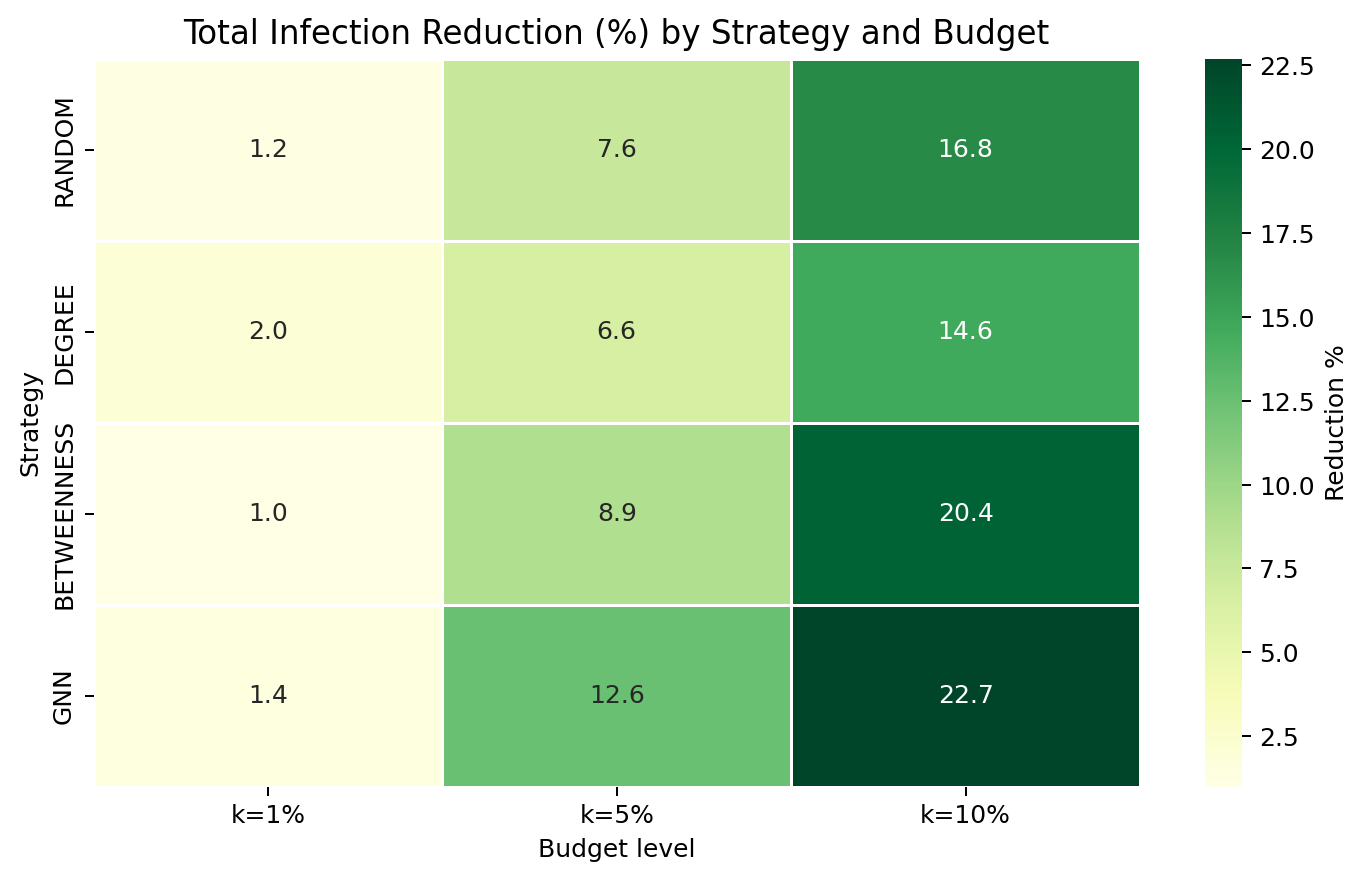
\includegraphics[width=\textwidth]{chart_heatmap.png}
  \caption{Counterfactual prevention rate.}
\end{subfigure}
\hfill
\begin{subfigure}{0.48\textwidth}
  \centering
  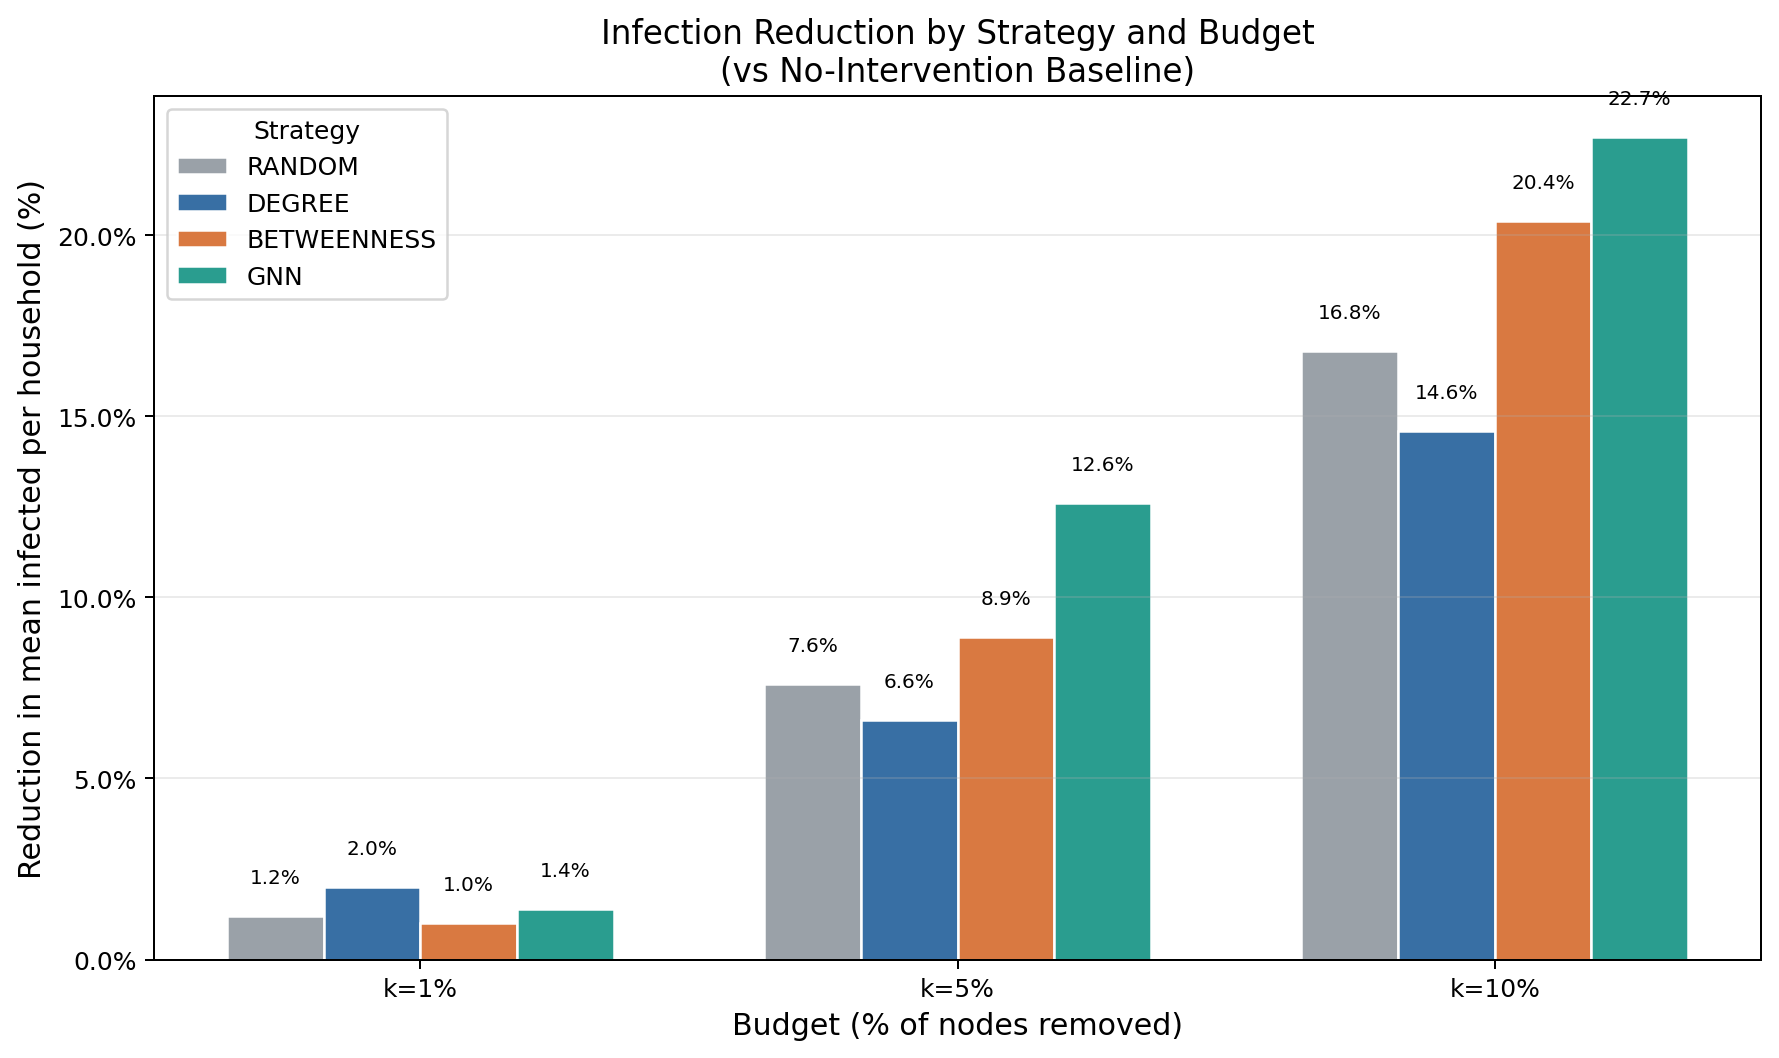
\includegraphics[width=\textwidth]{chart_reduction_by_strategy.png}
  \caption{SIR reduction by strategy.}
\end{subfigure}
\caption{Budget-dependent intervention performance. Source artifacts: \texttt{visualizations/chart\_heatmap.png} and \texttt{visualizations/chart\_reduction\_by\_strategy.png}.}
\label{fig:intervention-performance}
\end{figure}

\section{Discussion}

The results support a budget-sensitive interpretation of intervention strategy. When only three nodes can be selected, direct contact coverage is decisive, and Degree Centrality is a transparent and competitive heuristic. At the 5\% budget, GraphSAGE remains competitive after leakage control, but at the 10\% budget its counterfactual prevention rate no longer dominates the simpler baselines. This change is scientifically important: it indicates that the original node-level protocol overstated graph-learning performance, and that leakage-controlled household-held-out evaluation is necessary before making model-comparison claims.

Betweenness is weaker in this dataset because the graph is composed of disconnected household components. Bridge-like nodes are often important in networks with cross-community paths, but SASHTS contains no observed cross-household edges. This limits the value of global bridge-based intervention and shifts emphasis toward direct household exposure and local risk ranking.

These findings should be interpreted as evidence from a single household contact network. They do not establish universal superiority of graph learning for epidemic intervention. Instead, they suggest that simple centrality remains a strong and transparent baseline, while graph-learning rankings require stronger validation through repeated household-level folds and external datasets before they can support general recommendations.

\section{Limitations}

This study has several limitations. First, the dataset contains 340 individuals in 88 household components, which limits external validity for schools, workplaces, hospitals, or city-scale contact networks. Second, Klerksdorp records lack real timestamps, so the present analysis is static rather than fully temporal. Third, the Weighted GraphSAGE model is a proxy and not a full reproduction of DeepTrace. Fourth, Phase 03 removed the strongest identified leakage pathways, but remaining epidemiological variables still require source-level confirmation of observation timing. Fifth, the SIR model uses simplifying assumptions and has not yet undergone sensitivity analysis. Sixth, the intervention analysis assumes selected nodes can be fully removed or intervened on, which is not a validated public-health deployment model.

\section{Conclusion}

\costtrace\ demonstrates a reproducible graph-analysis workflow for budget-constrained intervention ranking in a household epidemic contact network. After Phase 03 leakage control, Degree Centrality remains strong under an extremely low budget, GraphSAGE is competitive at the 5\% budget, and no single strategy dominates all budgets and metrics. The manuscript should be considered a proof of concept until multi-fold household validation, sensitivity analyses, stronger baselines, and external datasets are added.

\section*{Ethics Statement}

This study is a secondary computational analysis of the SASHTS academic research dataset recorded in the local repository. The analysis does not recruit participants, contact individuals, or implement a real medical intervention. All reported results are aggregate graph, model, and simulation outputs. \TODO{Confirm original SASHTS ethics approval, consent terms, de-identification status, and whether the target journal requires the original approval identifier.}

\section*{Data Availability}

The local repository contains raw SASHTS files under \texttt{data/raw/}, processed graph artifacts under \texttt{data/processed/}, and generated metrics under \texttt{results/}. The public data-sharing statement cannot be finalized until raw-data redistribution permissions are confirmed. \TODO{Confirm the official SASHTS source URL/DOI, license/access terms, and whether raw files may be redistributed; if not, release code and non-sensitive derived artifacts only and direct users to the original data provider.}

\section*{Code Availability}

The analysis code is organized under \texttt{src/costtrace/}, with the main entry point \texttt{main.py}. Key result artifacts are stored under \texttt{results/}. \TODO{Insert final repository URL and commit hash for submission.}

\section*{Funding}

\TODO{Add funding statement or state that no external funding was received.}

\section*{Conflicts of Interest}

\TODO{Add conflict-of-interest statement for all authors.}

\section*{Author Contributions}

\TODO{Add author contribution taxonomy after final author order is confirmed.}

\section*{AI/Tool Use Disclosure}

Drafting and repository-upgrade assistance used AI coding tools inside the local development environment. All numerical claims in this manuscript are intended to trace to local code or generated artifacts. \TODO{Replace with the exact disclosure required by the confirmed target journal, including tool name/version if required.}

\begin{thebibliography}{99}

\bibitem{hamilton2017graphsage}
Hamilton WL, Ying R, Leskovec J.
Inductive representation learning on large graphs.
In: Advances in Neural Information Processing Systems. 2017;30.

\bibitem{blondel2008louvain}
Blondel VD, Guillaume JL, Lambiotte R, Lefebvre E.
Fast unfolding of communities in large networks.
Journal of Statistical Mechanics: Theory and Experiment. 2008;2008(10):P10008.

\bibitem{keeling2005networks}
Keeling MJ, Eames KTD.
Networks and epidemic models.
Journal of the Royal Society Interface. 2005;2(4):295--307.

\bibitem{kiss2017epidemics}
Kiss IZ, Miller JC, Simon PL.
Mathematics of Epidemics on Networks: From Exact to Approximate Models.
Springer; 2017.

\bibitem{freeman1977centrality}
Freeman LC.
A set of measures of centrality based on betweenness.
Sociometry. 1977;40(1):35--41.

\bibitem{newman2006modularity}
Newman MEJ.
Modularity and community structure in networks.
Proceedings of the National Academy of Sciences. 2006;103(23):8577--8582.

\bibitem{kermack1927sir}
Kermack WO, McKendrick AG.
A contribution to the mathematical theory of epidemics.
Proceedings of the Royal Society of London. Series A. 1927;115(772):700--721.

\bibitem{tan2025deeptrace}
Tan CW, Yu PD, Chen S, Poor HV.
DeepTrace: Learning to optimize contact tracing in epidemic networks with graph neural networks.
arXiv preprint. \TODO{Verify final publication metadata before submission.}

\bibitem{sashts}
Kleynhans J, et al.
SARS-CoV-2 household transmission study (SASHTS): physical proximity contact sensor data and epidemiological outcomes.
\TODO{Verify official dataset citation, DOI/URL, and access statement before submission.}

\end{thebibliography}

\end{document}
